\chapter{Campus Universitario}
\label{chap:Campus Universitario}

La Universidad Mayor de San Simón fue fundada mediante ley de 5 de noviembre de 1832 por el Mariscal Andrés de Santa Cruz. La misma ley dispuso la creación y funcionamiento de una Academia de Practicantes Juristas, con la que, en realidad, se inicia la Facultad de Derecho, y hasta la fecha la Universidad cuenta con 12 Facultades de las cuales 7 se encuentran dentro del campus. \cite{umss_history}

Actualmente dentro la página de la Universidad se puede encontrar un ``Mapa Universitario'', el cual se puede apreciar en la figura \ref{fig:mapa_old}, este mapa consiste en una vista del campus universitario como un todo dentro del plano de la ciudad de Cochabamba, la misma página cuenta con la sección ``Paseo Virtual'' la cual lamentablemente no muestra nada.\\

\begin{figure}[H]
  \begin{center}
    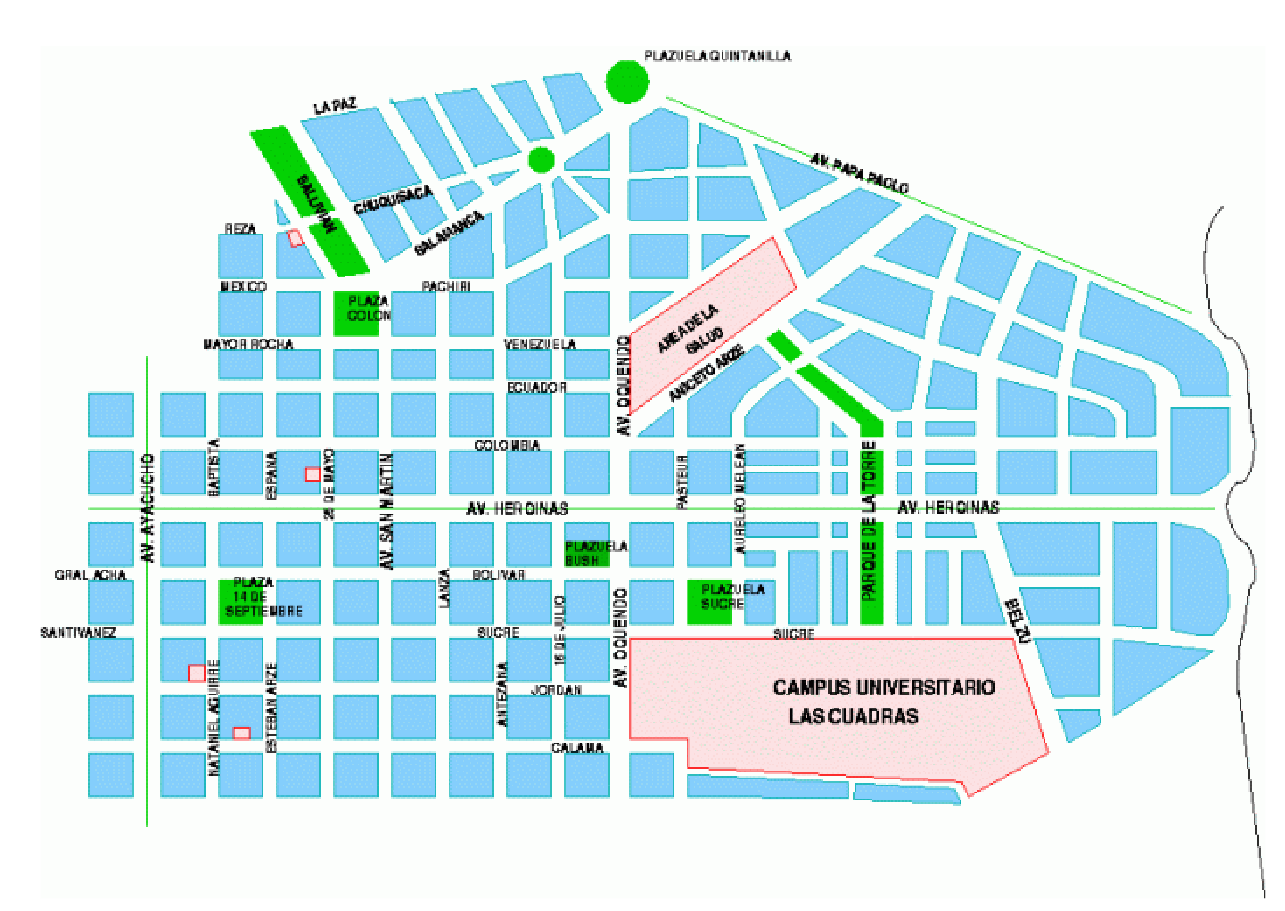
\includegraphics[width=0.75\textwidth]{mapa_old}
    \caption{Mapa universitario}
    \label{fig:mapa_old}
    \caption*{Fuente: \cite{umss_mapa}}
  \end{center}
\end{figure}


Como personas que usamos los predios del campus ya sea como estudiantes, docentes o visitantes, todos necesitamos contar con un mapa más actualizado del campus universitario.\\

Actualmente dentro del campus universitario ``Las Cuadras'' se encuentran las siguientes Facultades:

\begin{itemize}
\item FACH - Facultad de Arquitectura y Ciencias del Hábitat
% Dirección: Calle Jordán Interior
% Teléfonos: 4255730-4231172

\item FCJyP - Facultad de Ciencias Jurídicas y Políticas
% Dirección: Campus Central: Av. Oquendo esq Sucre
% Teléfonos: 591-4-4227509

\item FACES - Facultad de Ciencias Económicas
% Dirección: Edificio Prototipo I - Final Calama Este Campus Universitario
% Teléfonos: 4540245 - 4540248 - 4540261 FAX: 4540257


\item FHCE - Facultad de Humanidades y Ciencias de la Educación
% Dirección: Plaza Sucre acera Sud
% Teléfonos: 591-4-4544102

\item FCyT - Facultad de Ciencias y Tecnología
% Dirección: Calle Sucre y parque la Torre
% Teléfonos: 591-4-4231765

\end{itemize}

En la figura \ref, se puede apreciar a grandes rasgos la distribución de las facultados dentro del campus, un mapa nos sirve para darnos una idea hacia donde dirigirnos cuando queramos encontrar algún lugar dentro del campus universitario.\\


\begin{figure}[H]
  \begin{center}
    \label{fig:mapa_new}
    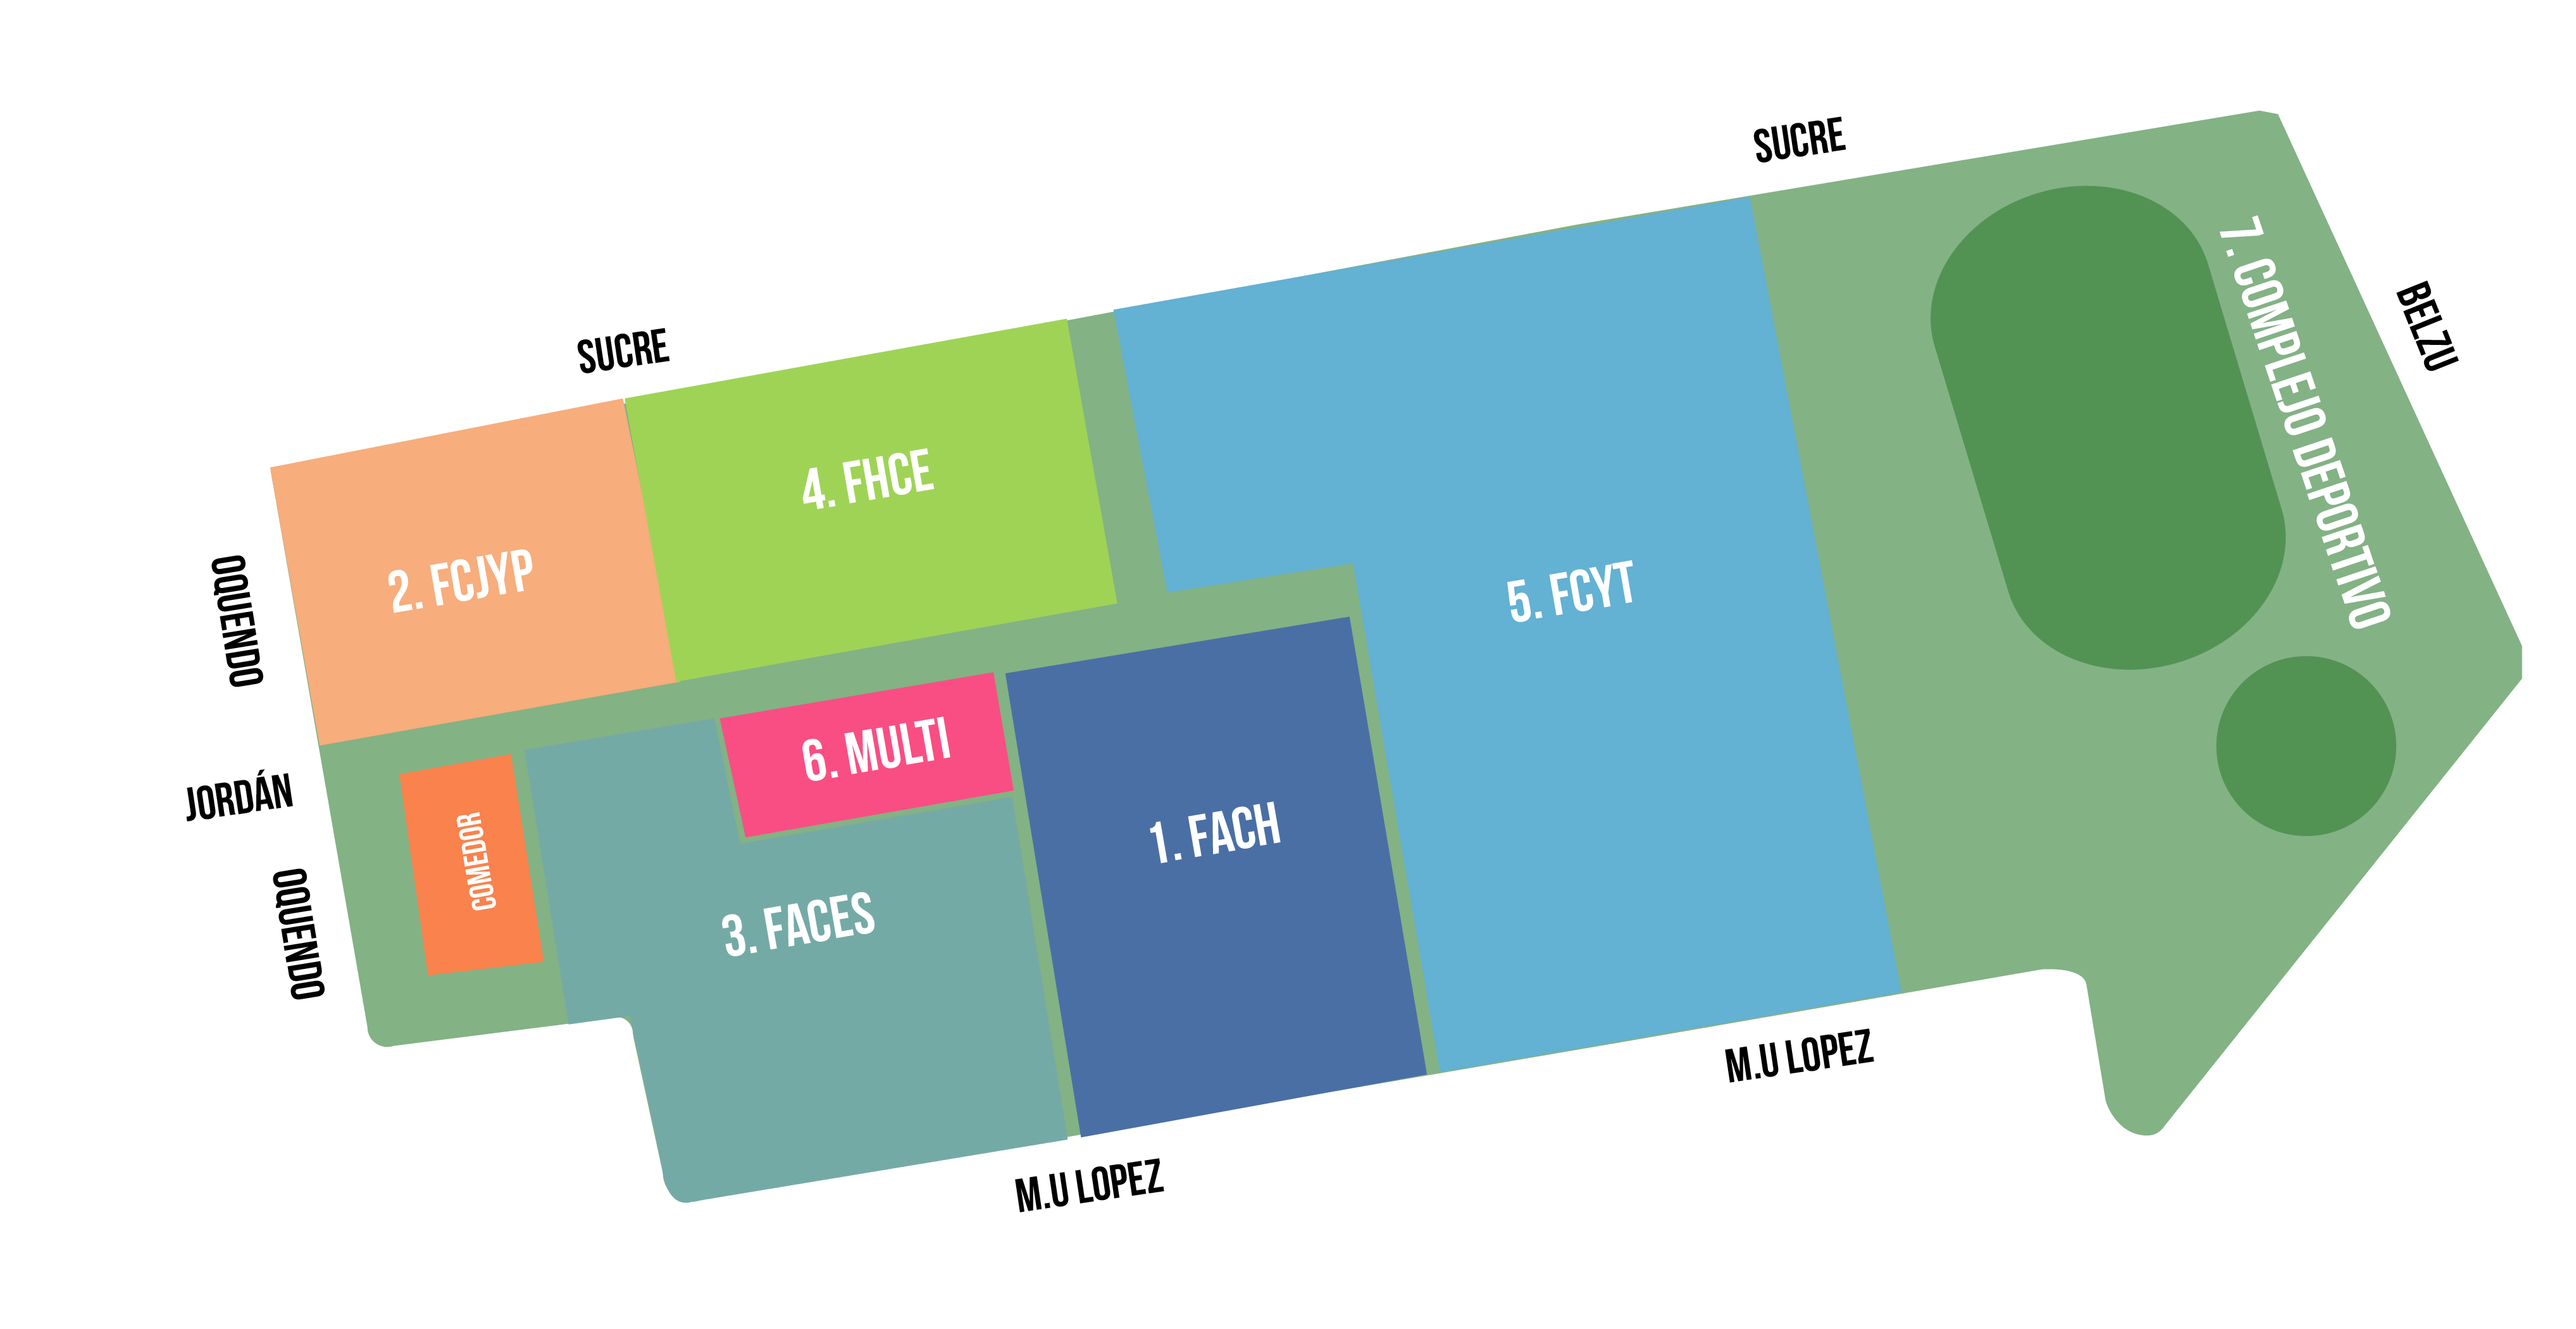
\includegraphics[width=1\textwidth]{mapa_new}
    \caption{Facultades dentro del Campus}
    \caption*{Fuente: Elaboración propia}
  \end{center}
\end{figure}

Pero no es suficiente ya que la Universidad cuenta con más de 600 Aulas y 200 oficinas y para un estudiante que pasa gran parte de su tiempo dentro del campus es difícil encontrar un lugar cuando no se sabe su locación exacta, para un visitante esto puede llegar a ser un gran problema.\\

Entonces conocer con exactitud la locación de un lugar es de gran importancia, para lo cual a continuación se detalla las locaciones por Facultad.

\section{Facultad de Arquitectura y Ciencias del Hábitat}
\label{sec:facultad_arquitectura}

% Dirección: Calle Jordán Interior
% FACH - Facultad de Arquitectura y Ciencias del Hábitat
    La Facultad de Arquitectura y Ciencias del Hábitat colinda con la calle M. U. Lopez, dentro de los predios del campus Universitario se halla entre las facultades de Economía hacia el Sur-Este y con la facultad de Tecnología hacia el Nor-Oeste, en la figura \ref{fig:fac_arqui} se puede apreciar la facultad con las aulas y oficinas que cuenta en su interior.

    \begin{figure}[H]
     \begin{center}
       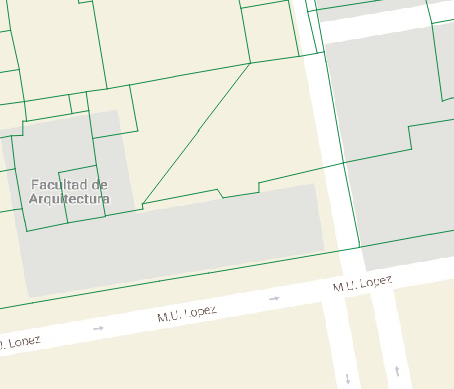
\includegraphics[width=0.75\textwidth]{fac_arqui}
       \caption{Facultad de Arquitectura - UMSS}
       \label{fig:fac_arqui}
       \caption*{Fuente: Elaboración propia}
     \end{center}
    \end{figure}


 \section{Facultad de Ciencias Jurídicas y Políticas}
 \label{sec:facultad_derecho}

 % La facultad de Derecho cuenta con alrededor de 178 vértices y 88 aristas, está ubicada al nor-oeste del Campus Universitario, en la esquina de la calle Oquendo y Sucre, dentro del campus colinda con la facultad de Humanidades hacia el Nor-Este y hacia el Sur-Oeste está la facultad de Economía.

 Generalmente conocida como ``Facultad de Derecho'' se encuentra al nor-oeste del Campus Universitario, en la Av. Oquendo esquina Sucre. En la figura \ref{fig:fac_derecho} se puede ver las locación de los lugares que se puede encontrar dentro de esta facultad.

 \begin{figure}[H]
   \begin{center}
     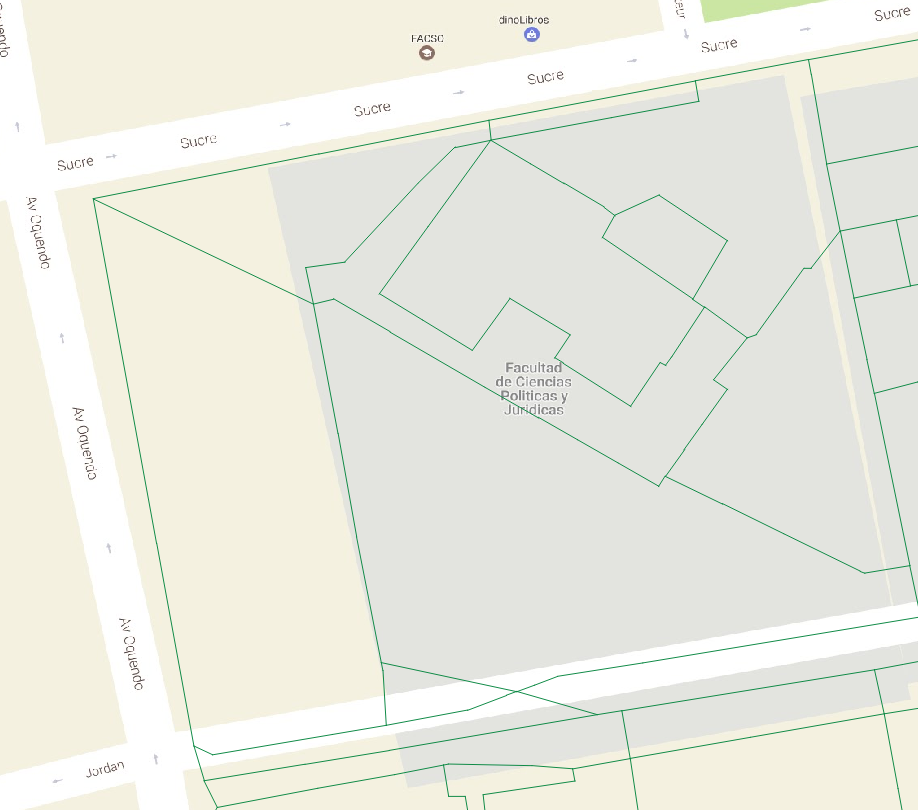
\includegraphics[width=0.5\textwidth]{fac_derecho}
     \caption{Facultad de Derecho - UMSS}
     \label{fig:fac_derecho}
     \caption*{Fuente: Elaboración propia}
   \end{center}
 \end{figure}

 \begin{table}[H]
  \begin{center}
    \begin{tabularx}{\textwidth}{ c  X }
      \toprule
        \textbf{Punto} &
        \textbf{Detalle}\\

      \midrule
        \textbf{1}
        &
        Centro de Estudiantes de Derecho
        \\

      \addlinespace
      \textbf{2}
      &
      1{\tiny er} Piso - Aula PP1, Aula PP2, Aula PP3, Aula PP4, Aula PP5, Aula PP6
      \\

      \addlinespace
      \textbf{3}
      &
      2{\tiny do} Piso - Aula SP1, Aula SP2, Aula SP3, Aula SP4, Aula SP5
      \\

      \addlinespace
      \textbf{4}
      &
      3{\tiny er} Piso - Carrera de Ciencia Politica
      \\

      \addlinespace
      \textbf{5}
      &
      3{\tiny er} Piso - Aula TP1, Aula TP2, Aula TP3, Aula TP4, Aula TP5
      \\

      \addlinespace
      \textbf{6}
      &
      3\text{\tiny er} Piso - Salon Auditorio ``Lic. Orlando Mercado Camacho''
      \\


      \addlinespace
      \textbf{7}
      &
      4{\tiny to} Piso - Aula CP1, Aula CP2, Aula CP3, Aula CP4, Aula CP5
      \\

      \addlinespace
      \textbf{8}
      &
      5{\tiny to} Piso - Aula QP1, Aula QP2, Aula QP3, Aula QP4, Aula QP5, Aula QP6
      \\

      \addlinespace
      \textbf{9}
      &
      Aula BA1
      \\

      \addlinespace
      \textbf{10}
      &
      Oficina Educativa Virtual Facultativa
      \\

      \addlinespace
      \textbf{11}
      &
      Full
      \\

      \addlinespace
      \textbf{12}
      &
      SITUMSS - Sindicato Trabajadores UMSS
      \\

      \addlinespace
      \textbf{13}
      &
      Snack Derecho
      \\

      \addlinespace
      \textbf{14}
      &
      Torre Fotos UMSS
      \\


      \bottomrule
    \end{tabularx}
    \caption{Locaciones de la Fac. Derecho}
    \label{tab:lugares_derecho}
  \end{center}
\end{table}




 % En la figura \ref{fig:fac_derecho} se puede observar en la línea verde los caminos o rutas dentro de la facultad de derecho de la UMSS, proyectada sobre el mapa de Google Maps, para lograr esta representación se utilizó QGIS ya que la información geográfica de la ruta está contenida en un archivo shapefile y el mapa se lo obtiene usando el API de Google Maps gracias al plugin de QGIS, \emph{QuickMapServices}.

 % \footnote{http://nextgis.com/blog/quickmapservices/}.




\section{Facultad de Ciencias Económicas}
\label{sec:facultad_economia}

      % Dirección: Edificio Prototipo I - Final Calama Este Campus Universitario
      La Facultad de Ciencias Económicas o comunmente conocida como ``Facultad de Economía'' está ubicada en el Edificio Prototipo I - Final Calama Este - Campus Universitario,

      colinda con las calles Oquendo y M. U. López, dentro del campus al Nor-Este se encuentra la facultad de Arquitectura y al Nor-Oeste la facultad de Derecho, tal como se puede apreciar en la figura \ref{fig:fac_economia}.

      \begin{figure}[H]
       \begin{center}
         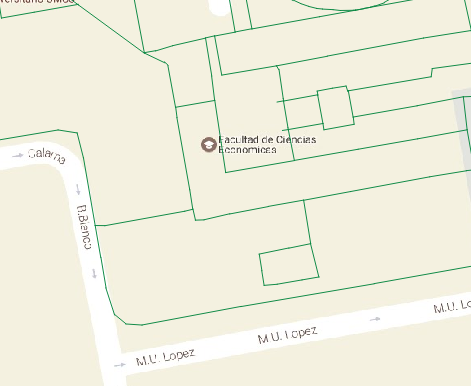
\includegraphics[width=0.75\textwidth]{fac_economia}
         \caption{Facultad de Economia - UMSS}
         \label{fig:fac_economia}
         \caption*{Fuente: Elaboración propia}
       \end{center}
      \end{figure}






\section{Facultad de Humanidades y Ciencias de la Educación}
\label{sec:facultad_humanidades}

La entrada a la facultad de Humanidades se lo encuentra sobre la calle Sucre en frente de la \emph{Plaza Sucre} acera Sud, en la figura \ref{fig:fac_humanidades} se puede apreciar la \emph{FHCE} dentro del campus Universitario la cual cuenta con XX oficinas y XXX aulas.

\begin{figure}[H]
 \begin{center}
   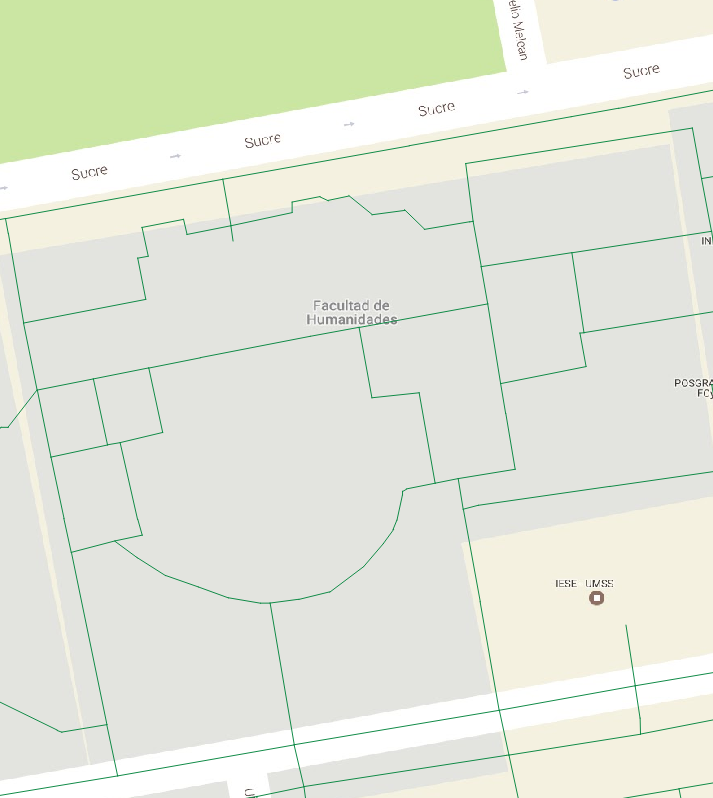
\includegraphics[width=0.75\textwidth]{fac_humanidades}
   \caption{Facultad de Humanidades - UMSS}
   \label{fig:fac_humanidades}
   \caption*{Fuente: Elaboración propia}
 \end{center}
\end{figure}


\section{Facultad de Ciencias y Tecnología}
\label{sec:facultad_tecnologia}

Comunmente conocida como ``facultad de Tecnología'',  se encuentra en el extremo Nor-Este dentro del campus Universitario, se puede encontrar una entrada a la facultad de tecnología sobre la calle  al frentre del parque \emph{la Torre} y otra entrada sobre la calle MU Lopez debajo de los edificios nuevos de tecnologia, dentro del campus Universitario colinda con las facultades de Arquitectura y Humanidades que se encuentran hacia el Sur-Este y Sur-Oeste correspondientemente, en la siguiente figura \ref{fig:fac_tecno} se puede apreciar la facultad de Tecnología con las locaciones de las xXX oficinas y xXX aulas que estan ubicadas dentro de la facultad.

\begin{figure}[H]
 \begin{center}
   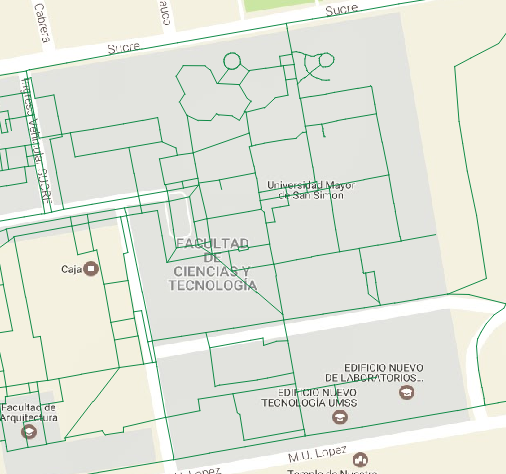
\includegraphics[width=0.75\textwidth]{fac_tecno}
   \caption{Facultad de Tecnología - UMSS}
   \label{fig:fac_tecno}
   \caption*{Fuente: Elaboración propia}
 \end{center}
\end{figure}

\section{Facultades fuera del campus Universitario}
\label{sec:Facultades fuera del campus Universitario}

Las siguentes facultades no se hallan dentro del campus Universitario ``Las Cuadras'' por lo que escapan del alcance del presente proyecto de grado, pero se las nombrara para el conocimiento del lector.

\begin{description}
  \item[FACSO:] La Facultad de Ciencias Sociales o ``SOCIOLOGIA'' esta ubicada Nataniel Aguirre No. S 0360 entre Santivañez y Jordán, tambien conocida como ``Campus Sociología''.
  \item[FByF:] Facultad de Ciencias Farmacéuticas y Bioquímicas ubicada sobre Av. Aniceto Arce frente Parque La Torre.
  \item[FCAPFyV:] Facultad de Ciencias Agrícolas, Pecuarias, Forestales y Veterinarias
  Facultad de Ciencias Agricolas, Pecuarias y Forestales ``Martin Cardenas'' (FCAPyP) ubicada en la Avenida Petrolera Km 5.
  \item[ODONTOLOGIA:] Facultad de Odontología aubicada dentro el ``Campus Salud'', Calle Venezuela y Av. Oquendo.
  \item[MEDICINA:] Facultad de Medicina ubicada en el ``Campus Salud'', Av. Aurelio Melean 379.
  \item[FPVA:] Facultad Politecnica del Valle Alto ubicada en la Av. Mayor Rocha Provincia Punata.
  \item[FDRyT:] Facultad de Desarrollo Rural y Territorial  ubicada en la Av. Petrolera Km 5.5 carretera antigua a Sta. Cruz. 

\end{description}

% \item SOCIOLOGIA - Facultad de Ciencias Sociales
% Dirección: Campus Sociología: Nataniel Aguirre No. S 0360 entre Santivañez y Jordán
% Teléfonos: 4502820 - 21 Fax: 4502821

% \item FByF - Facultad de Ciencias Farmacéuticas y Bioquímicas
% Dirección: Av. Aniceto Arce frente Parque La Torre
% Teléfonos: (591) (4) 420651 - (591) (4) 4250652


% FCAPFyV - Facultad de Ciencias Agrícolas, Pecuarias, Forestales y Veterinarias
%
% Dirección:
% Teléfonos: 4333808 - 4329666
%
% ODONTOLOGIA - Facultad de Odontología
%
% Dirección: Campus Salud: C. Venezuela y Av. Oquendo
% Teléfonos: 4530307 - 4530314
% Fax. 4530314
%
% MEDICINA - Facultad de Medicina
%
% Dirección: Campus Salud: Av. Aurelio Melean 379
% Teléfonos: 4231508 - 4254910
%
% FPVA - Facultad Politecnica del Valle Alto
%
% Dirección: Av. Mayor Rocha Provincia Punata
% Teléfonos: (591)(4) 4577299
%
% FDRyT - Facultad de Desarrollo Rural y Territorial
%
% Dirección: Av. Petrolera Km 5.5 carretera antigua a Sta. Cruz
% Teléfonos: 4762387 - Telefax: 4761983
